\section{Présentation de l'automate \textbf{LOGO} Siemens}



L'automate LOGO est un automate Monobloc de la marque Siemens. 
\textit{Monobloc} signifie qu'il contient nativement des entrées et des sorties directement sur le bloc de la CPU. 



\begin{UPSTIactivite}
    Un automate LOGO a été mis à votre disposition. Il est composé notamment de : 
    \begin{itemize}
        \item Deux bornes d'alimentation
        \item Huit entrées logiques
        \item Quatre sorties logiques à relais
        \item Une prise RJ45 pour se relier au réseau
        \item Une IHM composée de
        \begin{itemize}
            \item Un écran LCD
            \item Cinq boutons 
        \end{itemize}
    \end{itemize}

    \UPSTIquestion{Identifier les différents éléments composant la base du LOGO sur l'image suivante.}
    \UPSTIquestion{A l'aide de la documentation et de la référence sur le module, identifier et donner les caractéristiques des modules d'extension présents sur la maquette}

    \begin{center}
        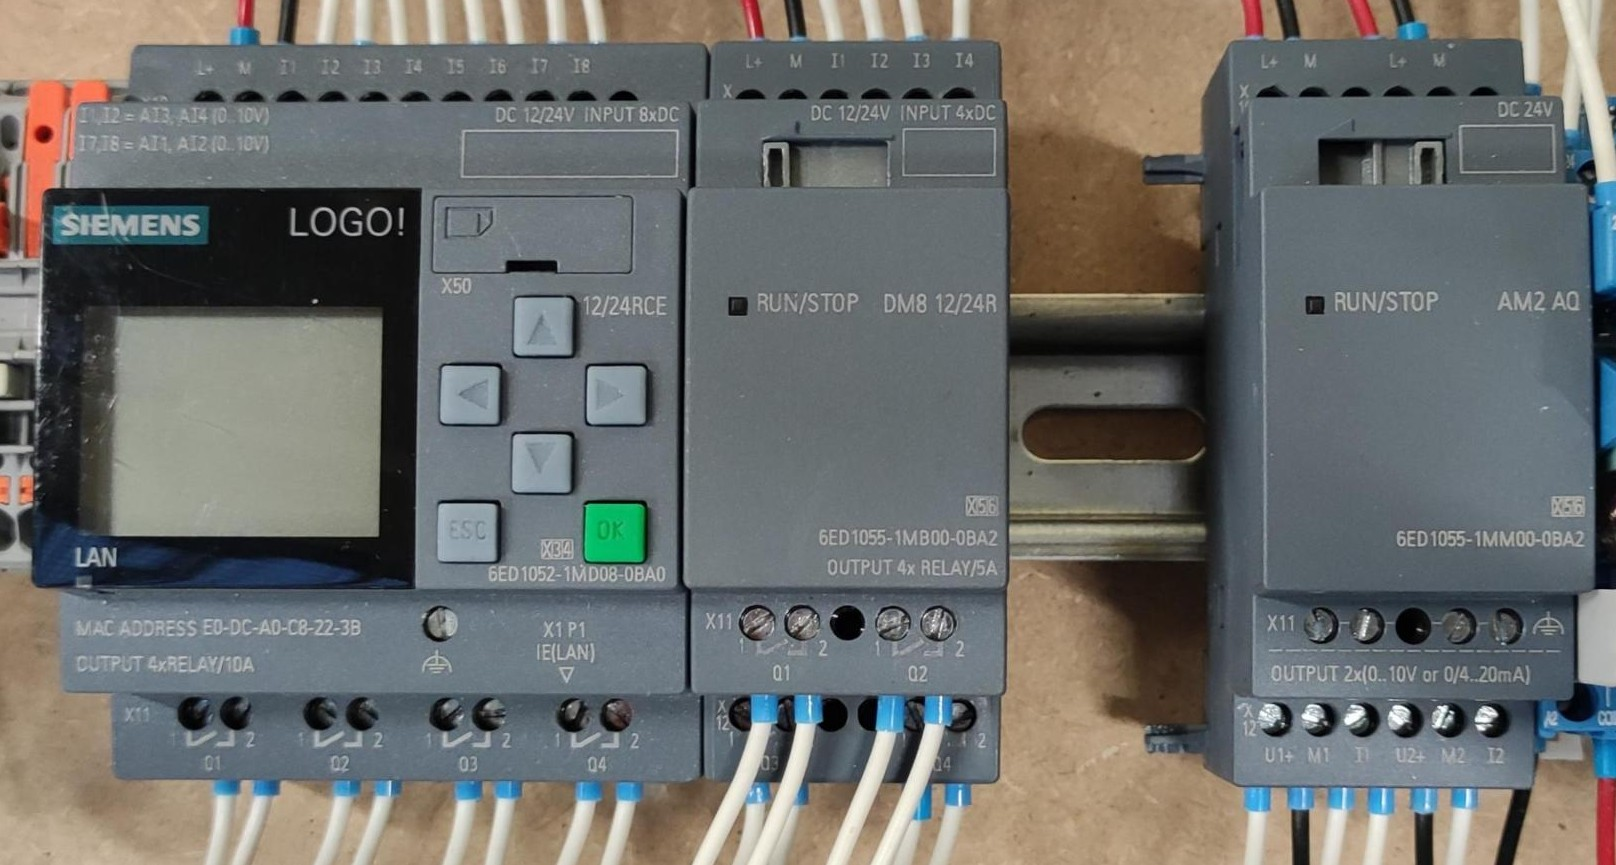
\includegraphics[width=.6\textwidth, height=.35\textheight,keepaspectratio]{images/maquette_logo.jpg}
    \end{center}

\end{UPSTIactivite}


